\section{Head coordinate system creation}
All the electrodes in the EEG cap have to be mapped to a single coordinate system. we will use BTi or 4D neuroimaging coordinate system defined as per \cite{BTi/4D}. The BTi/4D coordinate convention uses external anatomical features in the face such as the nasion, left, and right pre-auricular points (LPA \& RPA respectively) as a basis for the coordinate system as shown in \cref{fig:BTi_4D}. 

\begin{enumerate}
	\item The origin is between LPA \& RPA
	\item The $\vect{x}$ axis goes through nasion.
	\item The $\vect{y}$ goes through LPA, orthogonal to $\vect{x}$
	\item The $\vect{z}$ axis is orthogonal to both $\vect{x}$ \& $\vect{y}$
\end{enumerate}

\begin{figure}[hbt!]
	\centering
	\begin{subfigure}{0.49\textwidth}
		\includegraphics[width=\linewidth]{BTi_4D.png}
		\caption{The BTi/4D coordinate system convention.}
		\label{fig:BTi_4D_1} 	
	\end{subfigure}
	\hfill
	\begin{subfigure}{0.37\textwidth}
		\centering
		\includegraphics[width=\linewidth]{BTi_4D_2.png}
		\caption{Anatomical features of the face.} 
		\label{fig:BTi_4D_2}	
	\end{subfigure}
	\caption{Head coordinate system.}
	\label{fig:BTi_4D} 
\end{figure}  

fusionTrac 500 by Attarcsys along with marker is used to capture the points nasion, LPA, and RPA of the phantom head as shown in \cref{fig:BTi_4D_2} and the coordinate system is created using vector algebra. 

\begin{figure}[hbt!]
\centering
	\begin{subfigure}{0.35\textwidth}
		\includegraphics[width=\textwidth]{csys_1.png}
		\caption{Vectors in camera frame}
		\label{fig:csys_1}	
	\end{subfigure}
	\begin{subfigure}{0.35\textwidth}
		\includegraphics[width=\textwidth]{csys_2.png}
		\caption{Unit vector n}
		\label{fig:csys_2}	
	\end{subfigure}
	\\
	\begin{subfigure}{0.35\textwidth}
		\includegraphics[width=\textwidth]{csys_3.png}
		\caption{Unit vector $\vect{n}$, $\vect{V}_b - \vect{V}_a$ }
		\label{fig:csys_3}	
	\end{subfigure}
	\begin{subfigure}{0.35\textwidth}
		\includegraphics[width=\textwidth]{csys_4.png}
		\caption{vector $\vect{t}\  \&\  ((\vect{V}_b - \vect{V}_a).\vect{n})*\vect{n} $}
		\label{fig:csys_4}	
	\end{subfigure}
\caption{Vector algebra in head coordinate system creation.} 
\label{fig:BTi_4D_3}
\end{figure} 

The points a, b, c are nasion, LPA, RPA respectively in the camera coordinate system, vectors $ \vect{V}_a, \vect{V}_b, \vect{V}_c $ are created accordingly as depicted in \ref{fig:csys_1}. Then $\vect{V}_a - \vect{V}_p$ and an unit vector is computed from point a to b.

\begin{equation*}
\vect{n} = \frac{ {\vect{V}_{b} - \vect{V}_{a} } } {\| {\vect{V}_{b} - \vect{V}_{a} \|} }
\end{equation*}

\noindent The vector $\vect{V}_a - \vect{V}_p$ is then projected on to the unit vector $\vect{n}$ along point a, b and vector $\vect{t}$ is computed.

\begin{equation*}
Projection\  = ((\vect{V}_a - \vect{V}_p)n)*n)
\end{equation*}

\begin{equation*}
\vect{t} = (\vect{V}_a - \vect{V}_p) - (((\vect{V}_a - \vect{V}_p)n)*n)
\end{equation*}

we can calculate the origin of the coordinate system $ \vect{o} $ as 

\begin{equation*}
\vect{o} = \vect{V}_p + \vect{t}
\end{equation*}

its evident that $\vect{x}$ axis is along $\vect{t}$ but in a opposite direction. It is important to normalise $\vect{x}$ after computation.

\begin{equation*}
\vect{x} = - \vect{t} = - ((\vect{V}_a - \vect{V}_p) - (((\vect{V}_a - \vect{V}_p)n)*n))
\end{equation*}

\begin{equation}
\hat{\vect{x}} = -\frac{\vect{x}}{\| \vect{x} \|}
\end{equation}

similarly $\vect{y}$ axis and its normalised version can be computed as, 

\begin{equation*}
\vect{y} = - (\vect{V}_b - \vect{o})
\end{equation*} 

\begin{equation}
\hat{\vect{y}} = \frac{\vect{y}}{\| \vect{y} \|}
\end{equation} 
\noindent $ \hat{\vect{z}}$ is a vector cross product of $ \hat{\vect{x}}$ and $ \hat{\vect{y}}$

 
\begin{equation}
\hat{\vect{z}} = \hat{\vect{x}} \times \hat{\vect{y}}
\end{equation} 

\noindent A coordinate matrix can be created by combining $[\hat{\vect{x}}\  \hat{\vect{y}}\  \hat{\vect{z}}] $ also we can compute an orthonormal basis for this matrix using SVD.

\section{Electrode mapping} Having created a head coordinate system, we now present strategies for mapping all the electrodes in the EEG cap. Please note that the process of head coordinate system creation and electrode mapping are coupled and had to be done in the same setting without disturbing the head position but due to the limited working volume of the fusionTrac 500 camera as shown in \cref{fig:fusionTrac_phantom} it is evident that we cannot map all the electrodes in the cap without disturbing the head position especially the electrodes at the back of the head and this prompted to decouple the above 2 process. 

\begin{figure}[hbt!]
	\centering
	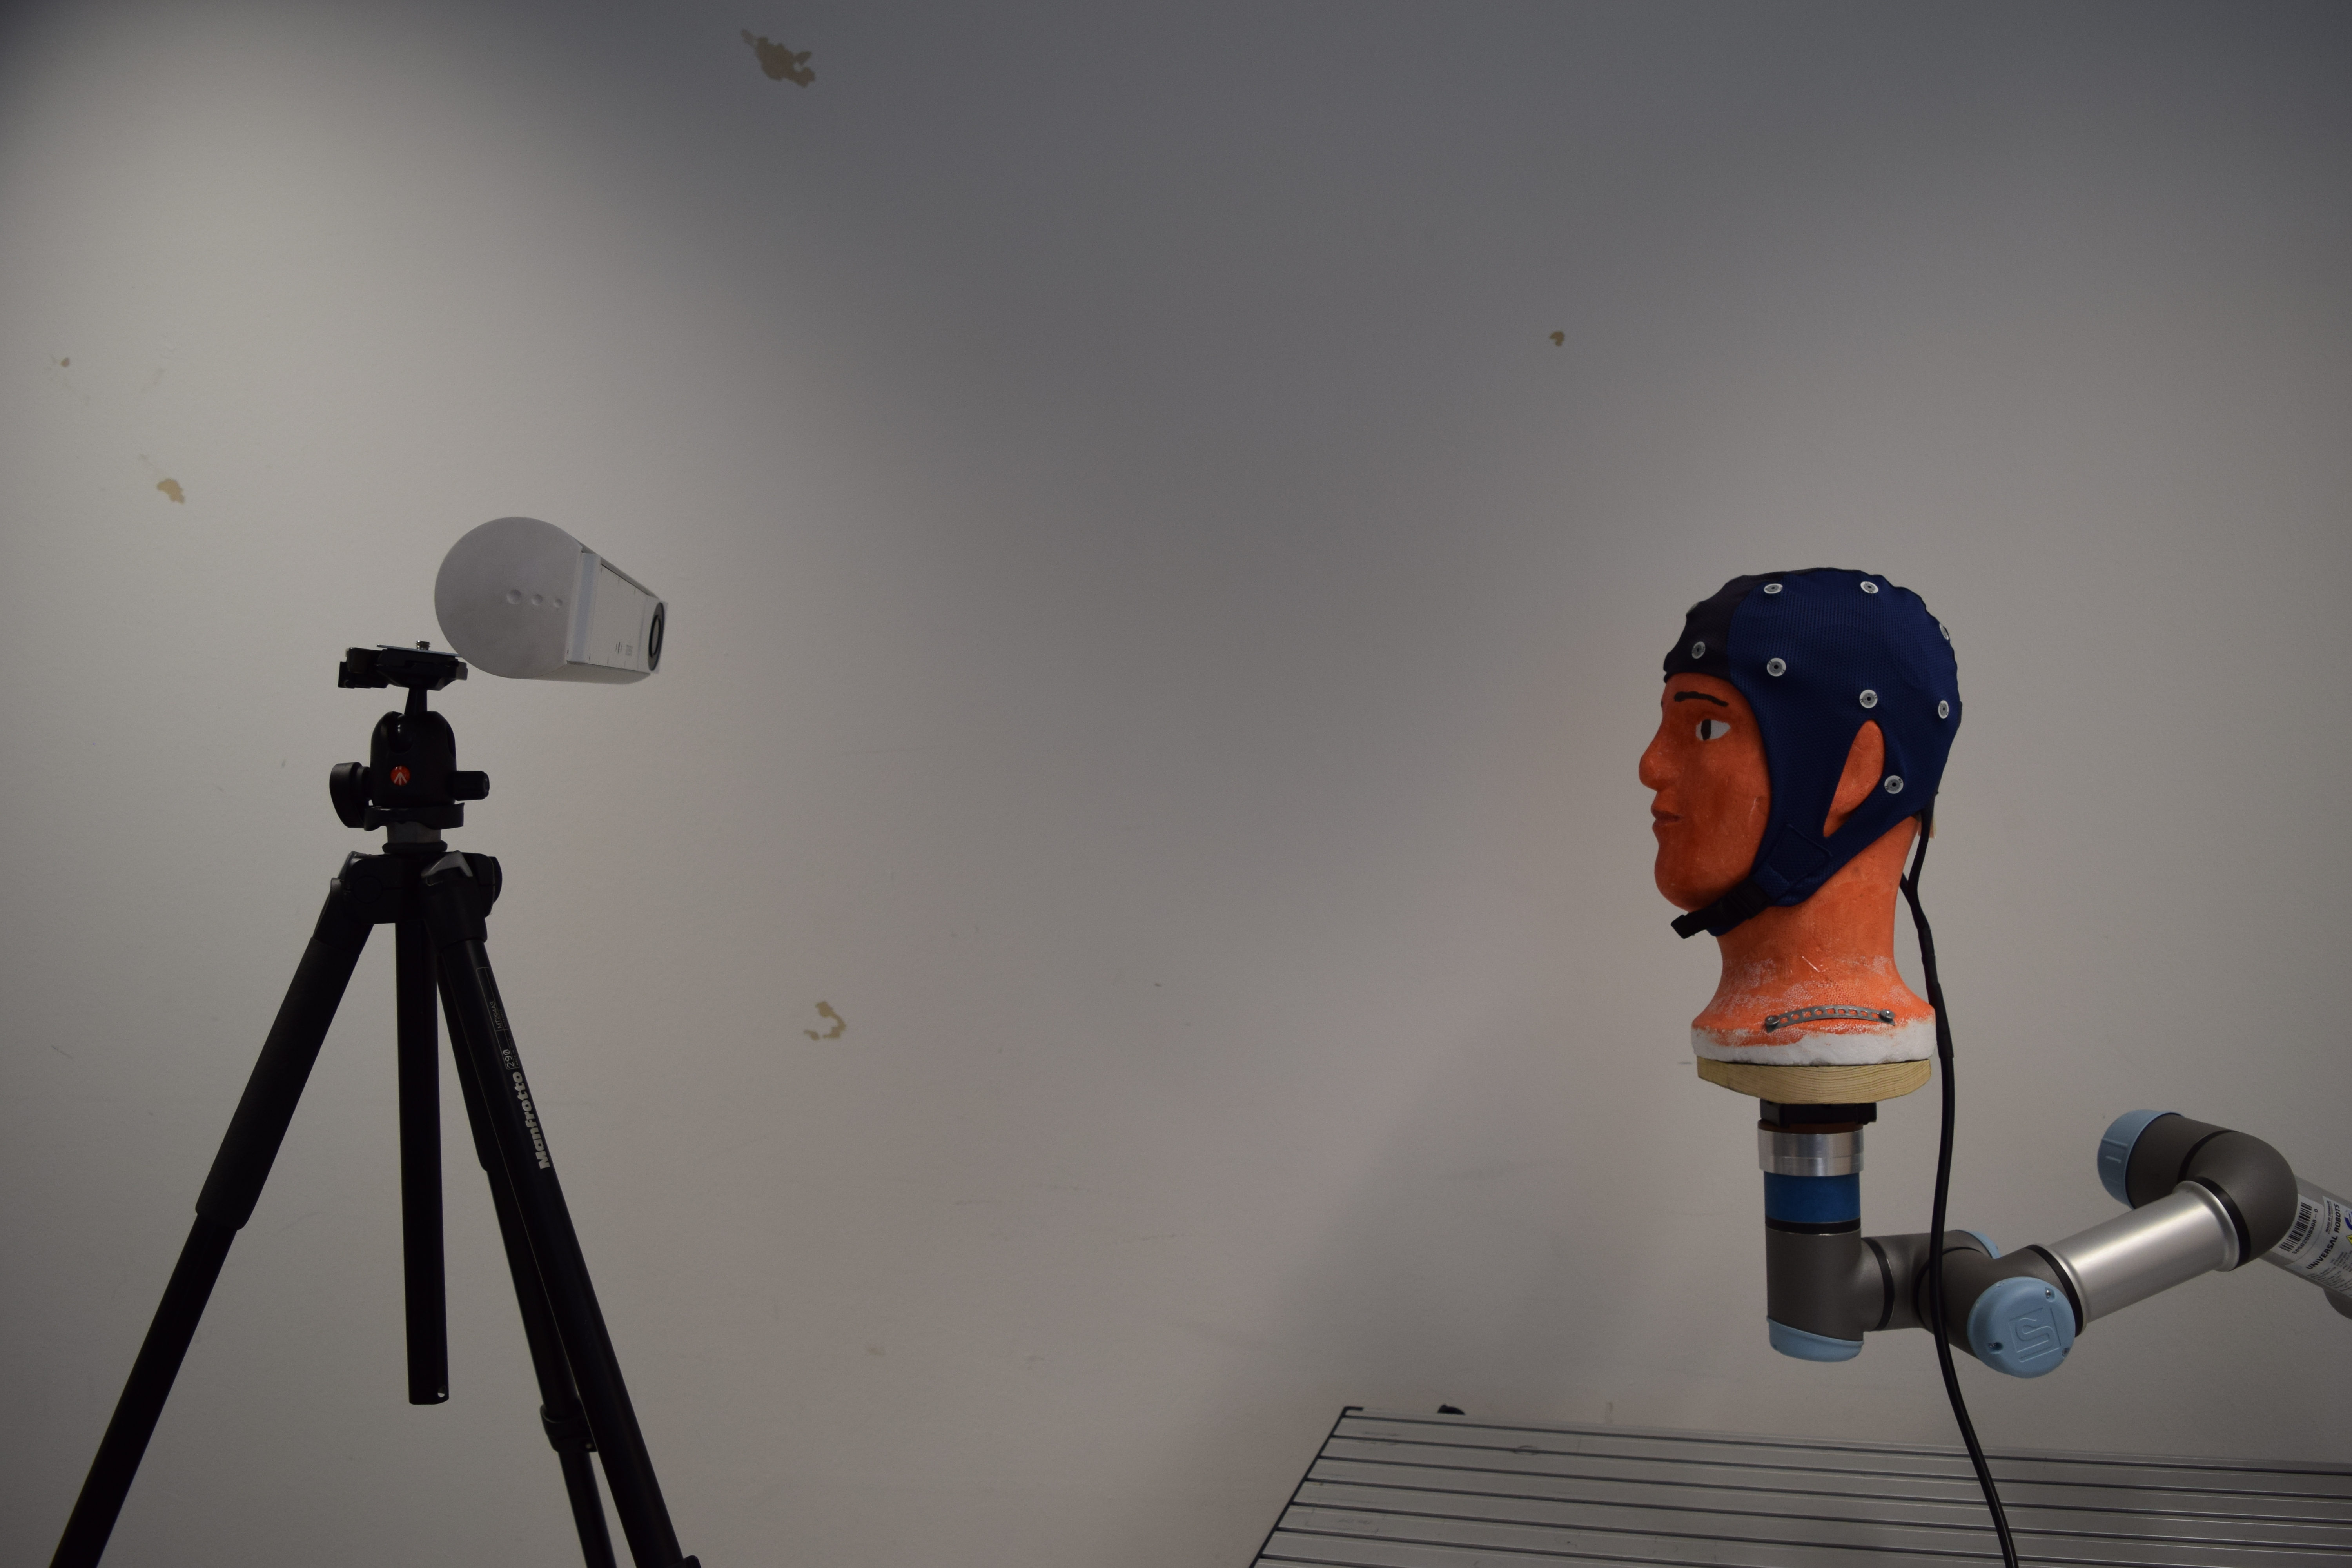
\includegraphics[scale=0.22]{fusionTrac_phantom.jpg}
	\caption{Difficult to capture electrodes at the back of the phantom head.} 
	\label{fig:fusionTrac_phantom}
\end{figure}

Decoupling can be achieved by mapping both the head coordinate system and electrode's position to a common frame of reference the one which we always know the position of. Robot's end-effector frame was selected as a frame of reference as we can enquire about the end-effector position via MoveIt. First, we will map the already created head coordinate system to robot end-effector $ \tfMat{EE}{T}{H_{cs}}$, let us recall the transformation between the camera and the robot's effector,

\begin{equation*}
\tfMat{EE}{T}{H_{cs}} = \invMat{(\tfMat{Base}{T}{EE})} \tfMat{Base}{T}{fCam} \tfMat{fCam}{T}{H_{cs}}
\end{equation*} 

where $\tfMat{Base}{T}{EE}$ is forward kinematics obtained via MoveIt, $\tfMat{Base}{T}{fCam}$ is evaluated via hand-eye calibration, $\tfMat{fCam}{T}{H_{cs}}$ is the head coordinate system created via fusionTrac 500 camera. The same process is applied for mapping the electrodes also. The advantage now is the head can be moved by commanding the robot until all the electrodes are covered.

\begin{equation*}
	\tfMat{EE}{T}{electrodes} = \invMat{(\tfMat{Base}{T}{EE})} \tfMat{Base}{T}{fCam} \tfMat{fCam}{T}{electrodes}
\end{equation*}  
Finally, all the electrodes can be mapped to head coordinate system via simple transformation.
\begin{equation*}
	\tfMat{H_{cs}}{T}{electrodes} = \invMat{(\tfMat{EE}{T}{H_{cs}})} \tfMat{EE}{T}{electrodes}
\end{equation*}

\section{Robot movement}
The phantom head wearing EEG is mounted to the robot and moved along spcified trajectories before recording the video in the Kinect camera. The \cref{fig:robot_movement} shows the robot movement along the single axis. The phantom is rotated 360 degrees clockwise first and then anti-clockwise in order to fully capture all the electrodes in the video thereby in the RGB images. 

\begin{figure}[hbt!]
	\centering
	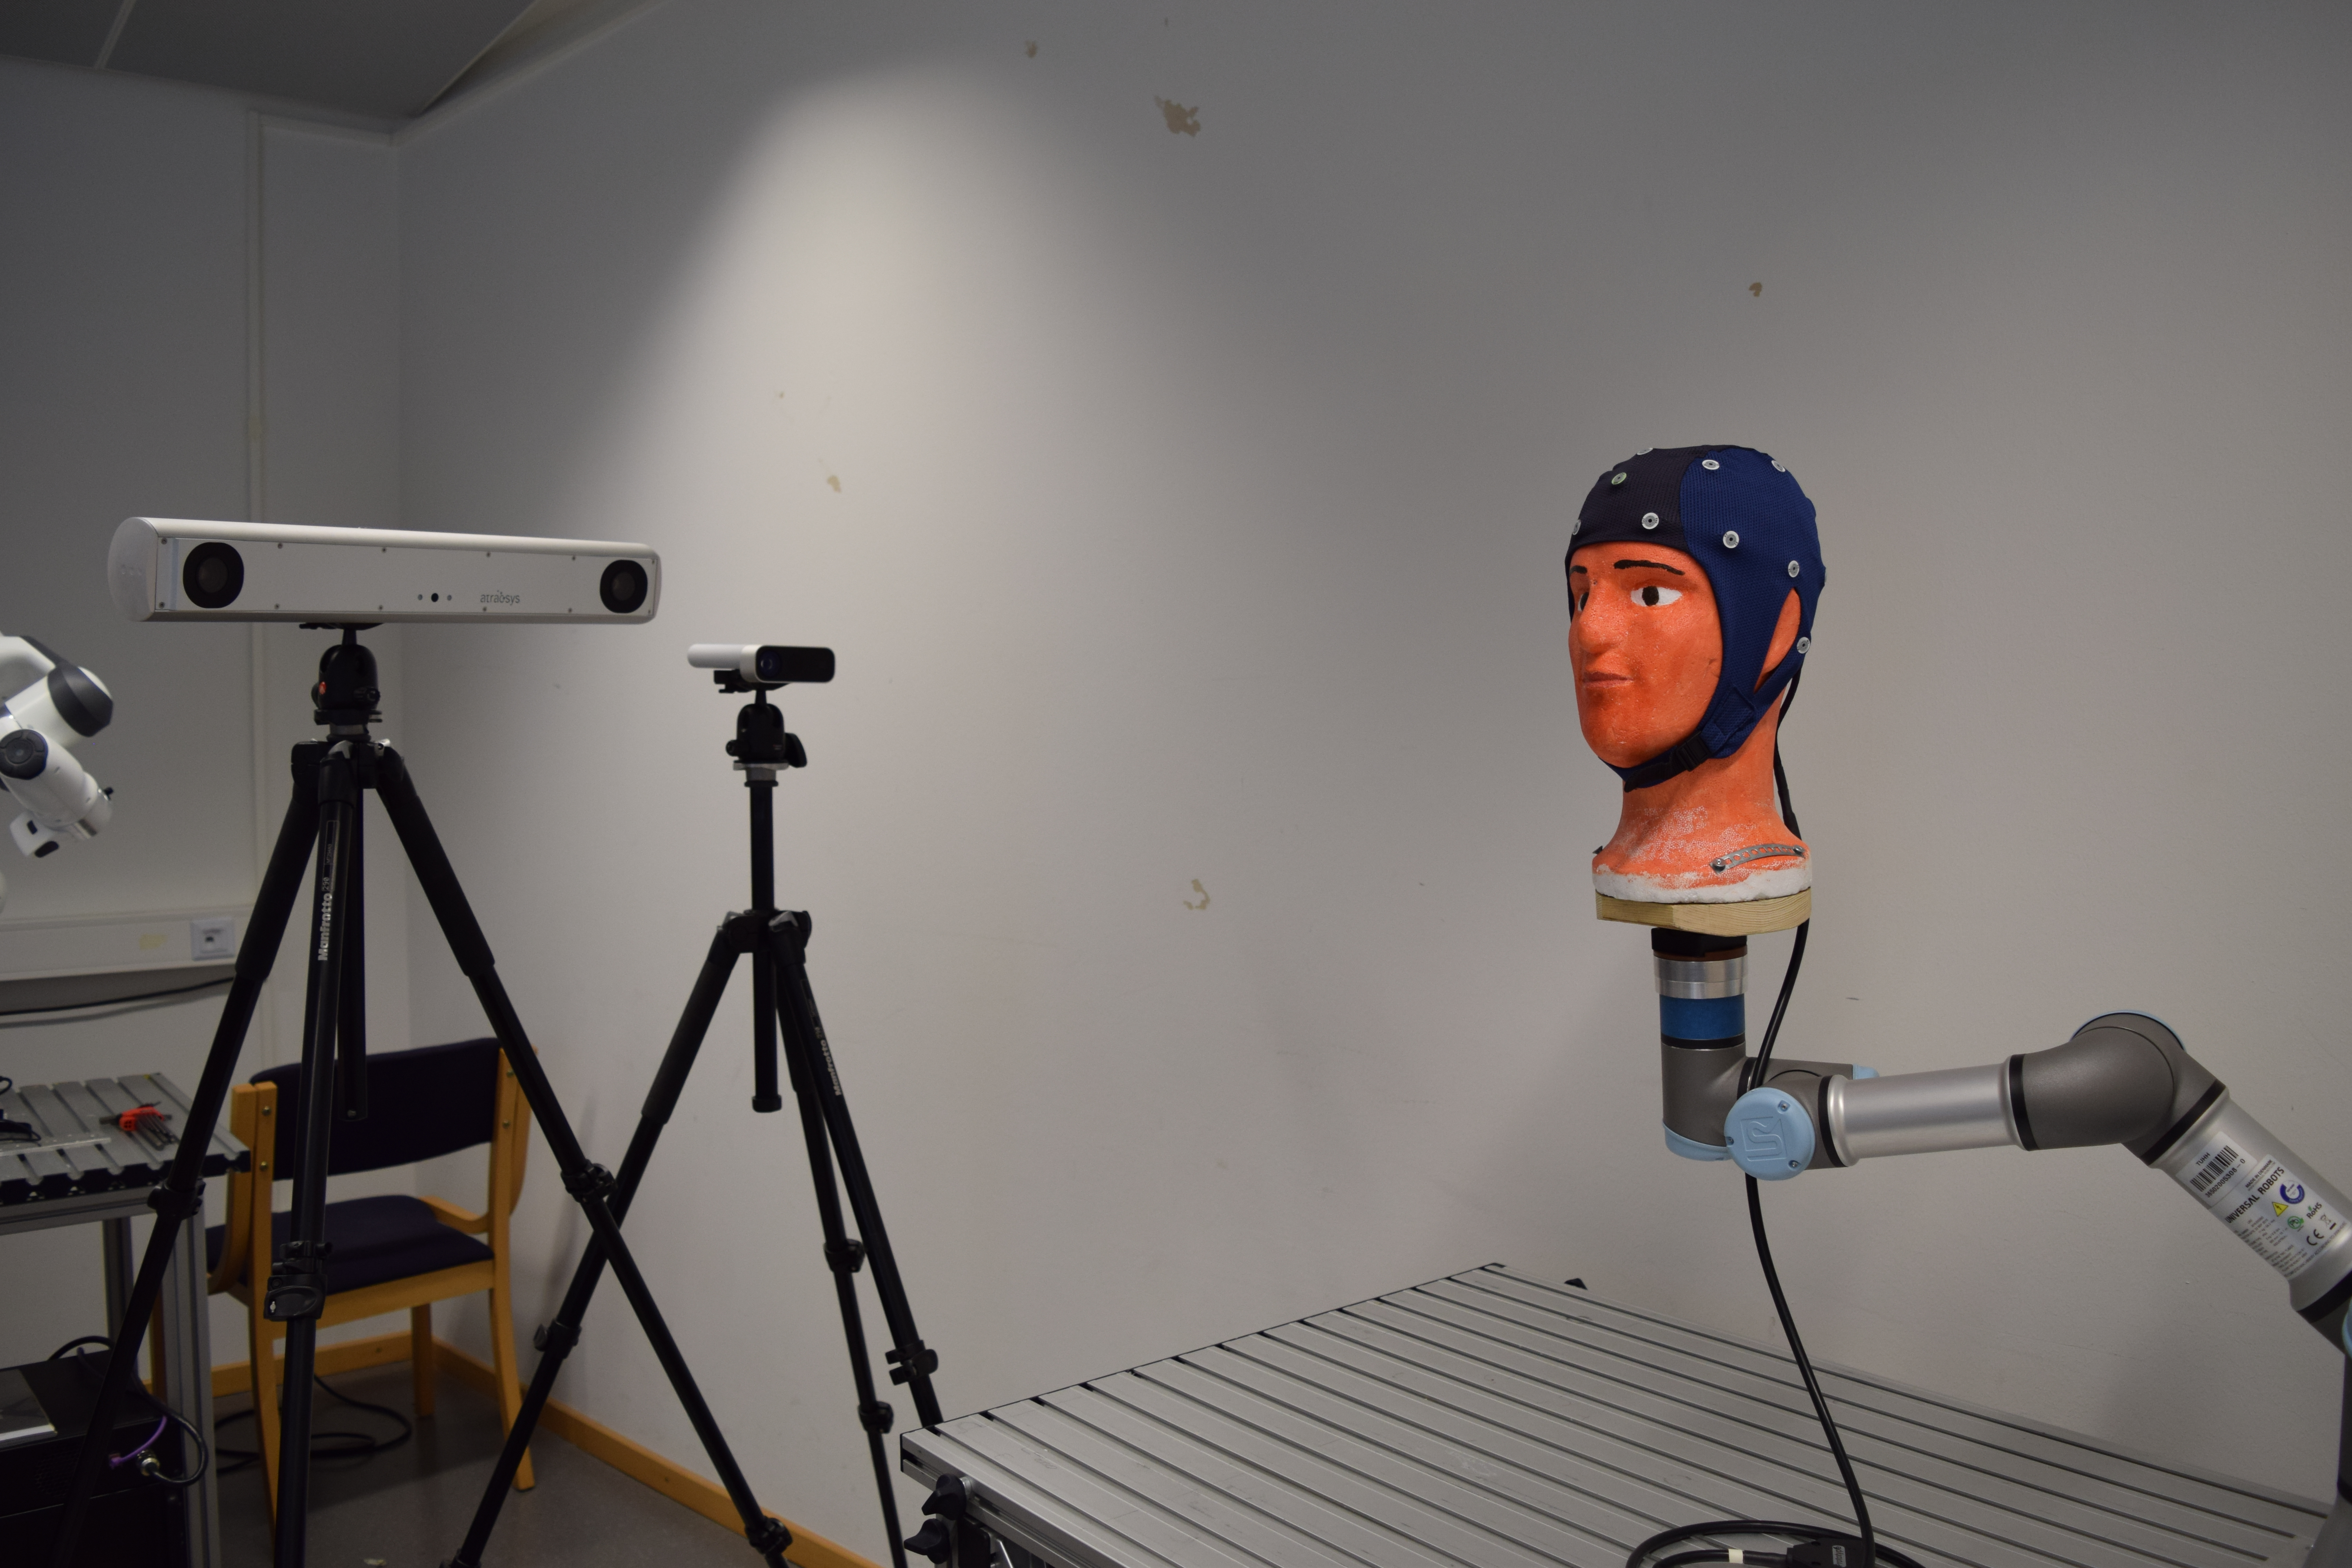
\includegraphics[scale=0.5]{robot_movement.png}
	\caption{360 degrees movement of the phantom head.} 
	\label{fig:robot_movement}
\end{figure}

\section{Ground truth data generation} 
Having electrode mapping strategy figured out, we are set to generate ground truth data generation and recording in Kinect frame.

\noindent\fbox{
	\parbox{\textwidth}{
		$\underline{Overview:}$\\ Here we would like to summarise all the steps involved in ground truth data generation.
		\begin{enumerate}
			\item Microsoft kinect :
				\begin{enumerate}
					\item Camera calibaration using chessboard.
					\item Hand-eye calibtaion using chessboard.
				\end{enumerate} 
			\item Atracsys fusionTrac 500 :
				\begin{enumerate}
					\item Hand-eye calibtaion using active marker.
					\item Head coordinate generation.
				\end{enumerate}
			\item Ground truth data recording in Kinect: 
				\begin{enumerate}
					\item Move the robot in a predetermined trajectory and while moving, record below highlighted ROS topics. 	
						\begin{enumerate}
							\item $/k4a/depth\_to\_rgb/camera\_info.$
							\item $/k4a/depth\_to\_rgb/image\_rect.$
							\item $/k4a/rgb/camera\_info.$
							\item $/k4a/rgb/image\_rect\_color.$
							\item $/k4a/points2.$
							\item $joints\_states.$
						\end{enumerate}
				\end{enumerate}
		\end{enumerate}
	}
}


\section{Accuracy of measurement}

While using the reflective marker, we are only interested in the tip position of the marker which is independent of the orientation of marker geometry. However, we tried to evaluate the calibration of the marker tip relative to the marker geometry by measuring the same electrode with 10 different orientations of the reflective marker and the error is recorded. 
 
Recall that we had to disturb the head position in order to map all the electrodes and we did it by introducing a common frame of reference i.e. robots end-effector frame at the cost of a measurement error. We also evaluated the positional error due to rotating head along a single axis and multiple axes to cover all electrodes. First, we rotated the phantom head to 10 different angles along a single axis while measuring the position of the single electrode at each of these 10 angles. Then, we repeated the same procedure but moved the phantom head along multiple axes as shown in \cref{fig:phantom_multiple_axis} and the positional error is recorded. 

\begin{figure}[hbt!]
	\centering
	\begin{subfigure}{0.49\textwidth}
		\includegraphics[width=\textwidth]{phantom_single_axis.png}	
	\end{subfigure}
	\hfill
	\begin{subfigure}{0.49\textwidth}
		\includegraphics[width=\textwidth]{phantom_multiple_axis.png}	
	\end{subfigure}
	\caption{Phantom head rotation along single and multiple axes.} 
	\label{fig:phantom_multiple_axis}
\end{figure} 

